\title{Lab 1: Intro to Arduinos \& Programming}
\author{Engineering 100-960/70}
\date{Fall 2020}
\documentclass[12pt]{article}
\usepackage[margin=1in]{geometry}
\usepackage{graphicx}
\usepackage{circuitikz}
\usepackage{fancyhdr}
\usepackage{hyperref}
\chead{Written \& Edited by }
\usepackage{hyperref}

\begin{document}
	\maketitle
	\thispagestyle{fancy}
	
	\section*{Materials}
	\begin{itemize}
		\item 1 \quad Arduino NANO 33 BLE Sense and cable
		\item 9 \quad LEDs (any color)
		\item 1 \quad 2-k$\Omega$ Resistor
	\end{itemize}
	
	\section*{Introduction}
	Welcome to the first lab of Engineering 100! In the initial labs in this course, we will focus on building technical understanding and skills in the areas of electronics, programming, and sensing. Our objective is for this knowledge to empower you for the design aspects of this course, as well as future courses in Michigan Engineering. To learn these fundamentals in the context of a project, you’ll be building a weather station that can measure temperature, relative humidity, and pressure.\newline
	
	The objective of lab 1 is learn how to power and command your Arduino. This entails some circuit building and some programming, but as you may have gathered from the pre-lab module, we’ll mostly focus on programming today. Next week, you’ll get a proper introduction to circuits. In the meantime, follow along with the lab manual, do not get discouraged, and DO ask the IAs what questions you have. They are here to help you learn and explore what piques your interest! 

	\section*{Pre-Lab Activities}
	FIXME: Reference the to the module (if this is even necessary)
	
	\section*{TINKERCAD Version}
    If you have not yet received your kit in the mail, this lab may be completed virtually, for up to full credit, using a circuit simulator in TINKERCAD. The TINKERCAD version of this lab manual can be found FIXME and covers the same concepts and activities as this manual.

	\section*{In-Lab Activities}
	

	\subsection*{The Breadboard}
    Before we build any circuits, it’s important to understand the tools that you are working with. A breadboard is like an engineer’s canvas when it comes to creating circuits. Notice that your breadboard has enumerated rows and columns. As you can see in Figure 1, underneath that plastic grid, those rows and columns are actually strips of metal. Two electrical components that are inserted into the same row or column on a breadboard will be \textbf{electrically connected}. This means that if, for instance, you connect a 5V battery to a given hole, all of the holes in that row have a voltage of 5V. In this way, devices can be chained together to create complex circuits. If you want to read more, feel free to check out this crash course on breadboards here: \url{https://www.makeuseof.com/tag/what-is-breadboard/}\newline
    	
    \begin{figure}[h!]
    	    \begin{center}
			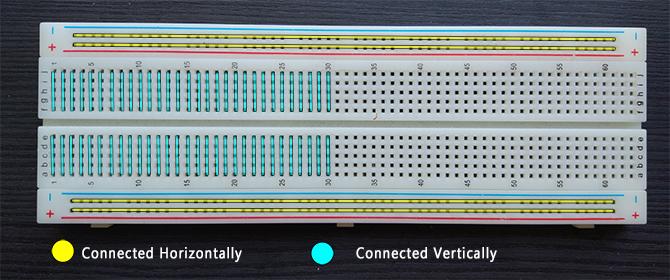
\includegraphics[width=\linewidth]{Figures/breadboard_annotated_670-1.jpg}
			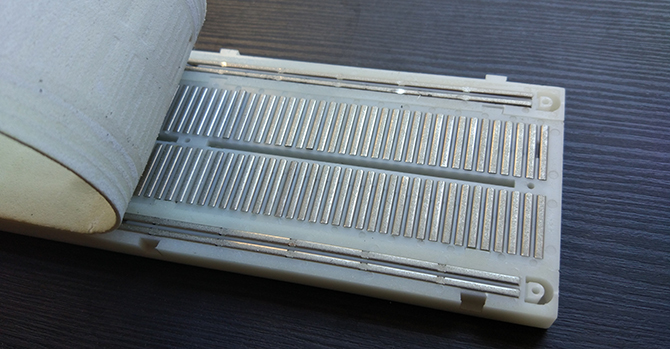
\includegraphics[width=\linewidth]{Figures/breadboard_back_peel_670.jpg}
			\caption{A breadboard, annotated (above) and with the plastic cover removed (below).\newline  \href{https://www.makeuseof.com/tag/what-is-breadboard/}{Credit: Makeuseof.com}}
		\end{center}
    	\end{figure}
    	
    The little legs on the Arduino are called \textbf{headers}, which are metal pins that can be inserted into the breadboard. The LEDs and resistors that you’ll use today are also made in a form that can be used with a breadboard. You'll be building the circuit show in Figure 2 momentarily. \newline
    	
    \begin{figure}[h!]
    	   **TODO: insert schematic and/or pic here of a single LED, resistor, and arduino set up on a breadboard**
    	   \caption{LED circuit to be built}
    \end{figure}
    	
    Pause and check-in with your group. What questions do you have about breadboards? What do you think an advantage is of prototyping with a breadboard is? Even if you have not worked with electronics before, can you think of any disadvantages?
    	
    \subsection*{Arduino Blink}
    Let’s try making first contact with the Arduino!
    \begin{enumerate}
	
	\item Insert the Arduino into the breadboard as you see in Figure 2. Don't add the LED and resistor just yet. Notice how it sits over the gap between the two columns on the breadboard. This positioning is intentional - if we placed the Arduino on one side of the breadboard, we would be electrically connecting pins on either side of the device. We don't know what this would do, and we want to make room to plug in other electronic devices, so as a result we place the Arduino in the center of the breadboard.
		    
	\item Turn on the Arduino by plugging in the micro USB cable into the device and the USB cable into your computer. Note that an LED built into the device should begin glowing. 
		    
    \item Load the Arduino Blink sketch in your IDE (sketch = nickname for an Arduino program).
    \begin{enumerate}
    	\item If you downloaded the Arduino Integrated Development Environment (IDE), first specify the Arduino model that you are working with by navigating to Tools $\rightarrow$ Board $\rightarrow$ Arduino Nano 33 BLE. Now, go to File $\rightarrow$ Examples $\rightarrow$ Basics $\rightarrow$ Blink.
        		    
        \item If you are using the Arduino Web Editor, first specify the Arduino model that you are working with by navigating to the dropdown menu labeled \textbf{Select Other Board \& Port}. Search and select \textbf{Arduino Nano 33 BLE}. Now, look to the left hand side and navigate to Examples $\rightarrow$ Basics $\rightarrow$ Blink.
    \end{enumerate}
    	        
    \item A new window should open up, with some code in it. In the lefthand corner of that window, click the checkmark to \textbf{compile} the program, and then click the arrow to \textbf{upload} the compiled program to the Arduino. Observe what happens on your Arduino.
    	 
    \textbf{ Troubleshooting:} If another LED on your Arduino does not begin blinking, try adjusting these settings, and then ask an IA:
    
    \begin{enumerate}
        \item If you downloaded the Arduino IDE, go to Tools $\rightarrow$ Port and select a different USB port on your computer, then re-upload the program. Try this on all available ports.
        \item If you are using the Arduino Web Editor, go to \textbf{Select Other Board \& Port} and select a different port for the Arduino Nano 33 BLE.
    	   \end{enumerate}
	   
    \end{enumerate}
        
    \subsection*{Arduino Programming Basics}
    Let's walk through the elements of the Arduino Blink sketch that you just ran. Every Arduino sketch consists of two functions: \verb|setup()| and \verb|loop()|. Try opening a new Arduino sketch (File $\rightarrow$ New) and you’ll notice that these functions are always provided to you as the starting point. 
        
    \begin{itemize}
    \item The \verb|setup()| function runs once when you upload a sketch to the Arduino, power the board, and/or press reset (see if you can find the reset button on your Arduino).
        
            \item The \verb|loop()| function runs “over and over again forever” – or at least until you upload different code or remove it from its power source.
        \end{itemize}

        The Arduino stores the most recent program that has been uploaded to it in it’s memory. See this for yourself by unplugging the Arduino from your computer, plugging it back in, and watching it restart the activities from the Blink sketch Even though you can't see it happening on the hardware, the Arduino ran the \verb|setup()| function once and then proceeded to continuously run the \verb|loop()| function .\newline
        
        Pause here and discuss with your partner(s): In an Arduino sketch, what kinds of actions belong in a \verb|setup()| function versus a \verb|loop()| function?\newline
        
        The last bit of the Arduino IDE that should be highlighted is the black box at the bottom of the window known as the \textbf{terminal}. By now you've already seen a success message appear after the Blink sketch. Perhaps while getting that sketch to run, you saw some error messages in the terminal as well. Although at first glance the error messages can be nasty, they can be \textit{very} useful when debugging. Other programmers have crafted these messages to help you figure out what has gone wrong in your program. When you don't know where to begin, try pasting that error into your favorite search engine. There's a decent chance that you aren't the first one to encounter this error! 

       \subsection*{Arduino Documentation}
       As stated in the prelab, Arduino refers to a company that manufactures open-source electronics and the community of people that provide ways to use those electronics (website link here).\newline 

        The Arduino IDE provides a wide range of functions that can be used in your Arduino programs. All of these functions are documented on the Arduino website. Reading documentation to understand and use something made by someone else is a really important skill in engineering. Look up \verb|pinMode()|, \verb|digitalWrite()|, and \verb|delay()| on your favorite search engine and read the documentation. Between looking up functions, discuss how these functions are used in the Arduino Blink program. 

        
	   \subsection*{LED Blink}
	   Now we'll see how we can control an external LED using an Arduino.
	   \begin{enumerate}
        	\item Unplug your Arduino from your computer. It is good practice to never manipulate a circuit while power is being supplied to it.
        	\item Build the LED circuit shown in Figure 2. 
        	
        	\item Plug your Arduino back into your computer. 
        	
        	\item Notice that only the Arduino’s built-in LED is blinking. Let’s add some code to the Blink sketch so that both the Arduino’s LED and this new LED cooperate. Look at your circuit. Following the picture, you should have connected the LED to one of the Arduino’s 14 \textbf{digital} pins, which are labelled D1-D14. Figure out which digital pin your LED is connected to, and then add a line of code in the \verb|setup()| function to initialize the LED using the command \verb|pinMode(<Your pin number>, OUTPUT)|;
        	
        	\item Follow the same logic to add lines of \verb|digitalWrite()| for this additional LED to the \verb|loop()| function of your program.
        	
        	\item Test this code and make sure that both LEDs blink. Be aware that LEDs only turn on when placed in your circuit in the correct orientation. Try switching the orientation of your LED if it doesn't turn on at this point. Take note that one leg of the LED is longer than the other. This can help you remember the proper orientation in the future.
        	
        	\item Save your code and rename it to something more recognizable. It will be prudent to create a new folder on your computer to store these scripts for easy recollection later. You will be submitting this program, so make sure to keep it.
        	
        \end{enumerate}
        
        \subsection*{Knight Rider}
        Connect 8 more LEDs to the Arduino digital out pins and ground them with one resistor, like in Figure 3. Write a new Arduino script to approximate the behavior of the light in the beginning of the video below (so that the light shifts left and right at a constant speed). This program should be written with less than 20 lines in loop. Make sure to save this code, as you will be submitting it. You should have three separate programs saved so far. (\url{https://www.youtube.com/watch?v=FpyKlLuLbcs})
        
        \begin{figure}[h!]
    	   **TODO: insert schematic and/or pic here for knight rider**
    	   \caption{The Knight Rider circuit}
    \end{figure}
	
	\section*{Deliverables}
	Submit the following 3 deliverables to assignment 'Week 1 Postlab' on Canvas:
	\begin{itemize}
	    \item Screenshot of code for Arduino Blink with External LED (step no. FIXME)
	    \item Screenshot of code for Knight Rider (step no. FIXME)
	    \item Submit some kind of proof of discussion with partners?
	\end{itemize}
	
\end{document}

